\section*{Consigna}

\begin{enumerate}
    \item Teniendo la siguiente topología, asignar los diferentes espacios de red para cada subred si la dirección de la red es 195.42.40.0/22:
\end{enumerate}

\vspace{-\baselineskip}
\begin{figure}[H]
    \centering
    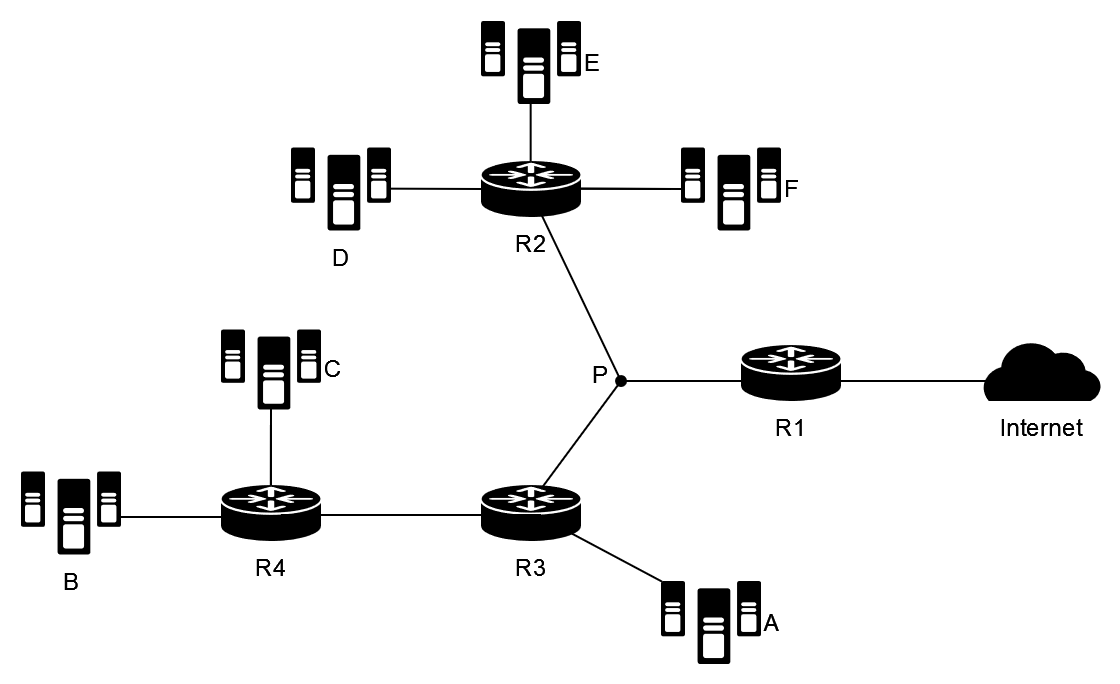
\includegraphics[width=1\linewidth]{Images/topologia.png}
\end{figure}

\vspace{-\baselineskip}
\begin{table}[H]
    \centering
    \begin{tabular}{|l|c|c|c|c|c|c|}
    \hline
    \multicolumn{1}{|c|}{Subnet} & A & B & C & D & E & F \\ \hline
    \#Hosts & \multicolumn{1}{r|}{126} & \multicolumn{1}{r|}{61} & \multicolumn{1}{r|}{500} & \multicolumn{1}{r|}{50} & \multicolumn{1}{r|}{30} & \multicolumn{1}{r|}{2} \\ \hline
    \end{tabular}
\end{table}

\begin{enumerate}[start=2]
    \item ¿Por qué se suma dos a la cantidad de direcciones?
    \item ¿Por qué los tamaños de bloque son potencias de 2?
    \item ¿Cuántas direcciones sin utilizar quedaron?
    \item De las direcciones sin utilizar ¿Cuántas son útiles?
    \item ¿Se puede agregar una subred de 200 hosts?
\end{enumerate}